\documentclass{beamer}
\usepackage[english, russian]{babel}
\usepackage[T2A]{fontenc}
\usepackage[utf8]{inputenc}
\usepackage{indentfirst}
\usepackage{amsmath, amsfonts, amssymb, amsthm, mathtools}
\usepackage[export]{adjustbox}
\usepackage{graphicx} 
\graphicspath{ {./images/} }

\usepackage{subcaption}
\usepackage{verbatim}

\usepackage{minted}{\setlength{\parskip}{0pt}}

\usepackage{hyperref}

\hypersetup{
    colorlinks=true,
    linkcolor=blue,
    filecolor=magenta,      
    urlcolor=black,
    pdftitle={Overleaf Example},
    pdfpagemode=FullScreen,
    }


\title{Отчет по лабораторной работе № 5. \\Расширенная настройка HTTP-сервера Apache }
\author{Данила Стариков \\ НПИбд-02-22}
\date{2024}

\begin{document}

\maketitle
\newpage

\tableofcontents

\newpage
\section{Цель работы}
Приобретение практических навыков по расширенному конфигурированию HTTP-сервера Apache в части безопасности и возможности использования PHP.
\newpage
\section{Выполнение работы}
\subsection{Конфигурирование HTTP-сервера для работы через протокол HTTPS}
\begin{enumerate}
\item Загрузили вашу операционную систему и перейдите в рабочий каталог с проектом:
\begin{minted}{bash}
cd /var/tmp/dastarikov/vagrant
\end{minted}
\item Запустили виртуальную машину server:
\begin{minted}{bash}
make server-up
\end{minted}
\item На виртуальной машине server вошли и открыли терминал. Перешли в режим суперпользователя:
\begin{minted}{bash}
sudo -i
\end{minted}
\item В каталоге \texttt{/etc/ssl} создали каталог private:
\begin{minted}{bash}
mkdir -p /etc/pki/tls/private
ln -s /etc/pki/tls/private /etc/ssl/private
cd /etc/pki/tls/private
\end{minted}
Сгенерировали ключ и сертификат, используя следующую команду:
\begin{minted}{bash}
openssl req -x509 -nodes -newkey rsa:2048 -keyout www.dastarikov.net.key -out www.dastarikov.net.crt
mv www.dastarikov.net.crt /etc/pki/tls/certs
\end{minted}

Далее заполнили сертификат (Рис. \ref{01}):
\begin{itemize}
    \item в строке кода страны укажите RU;
    \item в строке названия страны укажите Russia;
    \item в строке названия города укажите Moscow;
    \item в строке названия организации укажите свой логин;
    \item в строке названия подразделения укажите свой логин;
    \item в строке названия хоста должно быть указано доменное имя вашего веб-сервера dastarikov.net;
    \item в строке e-mail адреса должен быть указан dastarikov@dastarikov.net.
\end{itemize}
    
\begin{center}
    \centering
    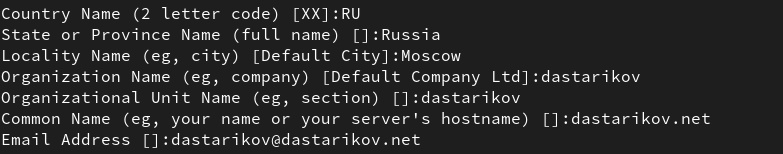
\includegraphics[width=\textwidth]{../images/image01.png}
    \captionof{figure}{Создание SSL-сертификата.}
    \label{01}
\end{center}

Сгенерированные ключ и сертификат появились в соответствующем каталоге \break\texttt{/etc/ssl/private}. Скопировали сертификат в каталог \texttt{/etc/ssl/certs}:

\begin{minted}{bash}
cp /etc/ssl/private/www.dastarikov.net.crt /etc/ssl/cert/
\end{minted}

\item Для перехода веб-сервера \texttt{www.dastarikov.net} на функционирование через протокол HTTPS изменили его конфигурационный файл. Перешли в каталог с конфигурационными файлами:
\begin{minted}{bash}
cd /etc/httpd/conf.d
\end{minted}
Открыли на редактирование файл \texttt{/etc/httpd/conf.d/www.dastarikov.net.conf} и заменили его содержимое на следующее (Рис. \ref{03}):
\begin{minted}{xml}
<VirtualHost *:80>
ServerAdmin webmaster@dastarikov.net
DocumentRoot /var/www/html/www.dastarikov.net
ServerName www.dastarikov.net
ServerAlias www.dastarikov.net
ErrorLog logs/www.dastarikov.net-error_log
CustomLog logs/www.dastarikov.net-access_log common
RewriteEngine on
RewriteRule ^(.*)$ https://%{HTTP_HOST}$1 [R=301,L]
</VirtualHost>
<IfModule mod_ssl.c>
<VirtualHost *:443>
SSLEngine on
ServerAdmin webmaster@dastarikov.net
DocumentRoot /var/www/html/www.dastarikov.net
ServerName www.dastarikov.net
ServerAlias www.dastarikov.net
ErrorLog logs/www.dastarikov.net-error_log
CustomLog logs/www.dastarikov.net-access_log common
SSLCertificateFile /etc/ssl/certs/www.dastarikov.net.crt
SSLCertificateKeyFile /etc/ssl/private/www.dastarikov.net.key
</VirtualHost>
</IfModule>
\end{minted}

Теперь при попытке подключиться по старому адресу через http будет происходить переадресация на соответствующие адреса https, за что отвечают команды:
\begin{minted}{xml}
RewriteEngine on
RewriteRule ^(.*)$ https://%{HTTP_HOST}$1 [R=301,L]
\end{minted}


Сами настройки подключения по протоколу HTTPS описаны внутри тега \texttt{<IfModule mod\_ssl.c>}, отличия есть только в наличии команды \texttt{SSLEngine on} и указания местоположения файла SSL-сертификата.

\begin{center}
    \centering
    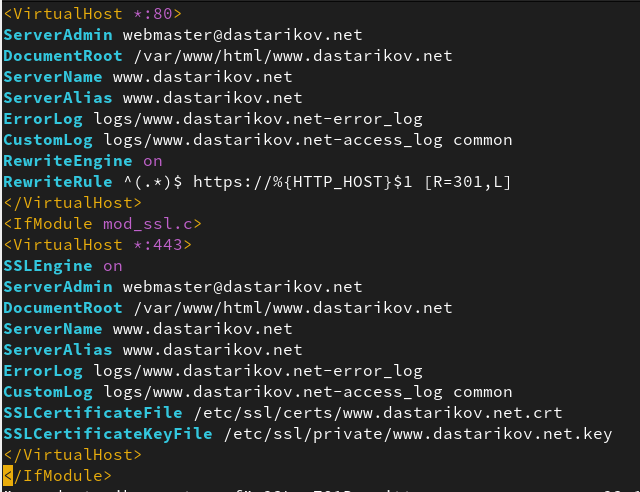
\includegraphics[width=\textwidth]{../images/image03.png}
    \captionof{figure}{Изменение конфигурационного файла для работы через протокол HTTPS.}
    \label{03}
\end{center}

\item Внесли изменения в настройки межсетевого экрана на сервере, разрешив работу с \texttt{https} (Рис. \ref{04}):
\begin{minted}{bash}
firewall-cmd --list-services
firewall-cmd --get-services
firewall-cmd --add-service=https
firewall-cmd --add-service=https --permanent
firewall-cmd --reload
\end{minted}

\begin{center}
    \centering
    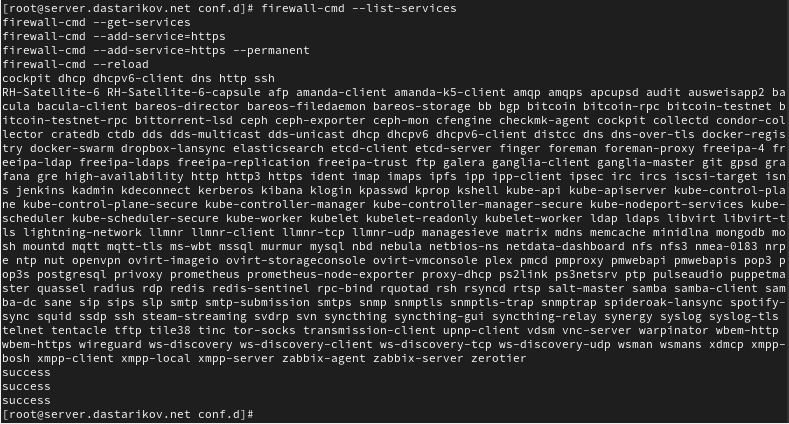
\includegraphics[width=\textwidth]{../images/image04.png}
    \captionof{figure}{Настройка межсетевого экрана.}
    \label{04}
\end{center}

\item Перезапустили веб-сервер:
\begin{minted}{bash}
systemctl restart httpd
\end{minted}
\item На виртуальной машине \texttt{client} в строке браузера ввели название веб-сервера \texttt{www.dastarikov.net} и убедились, что происходит автоматическое переключение на работу по протоколу HTTPS. На открывшейся странице с сообщением о незащищённости соединения нажали кнопку «Дополнительно», затем добавили адрес вашего сервера в постоянные исключения. Затем просмотрели содержание сертификата (нажмите на значок с замком в адресной строке и кнопку «Подробнее») (Рис. \ref{06}).

\begin{center}
    \centering
    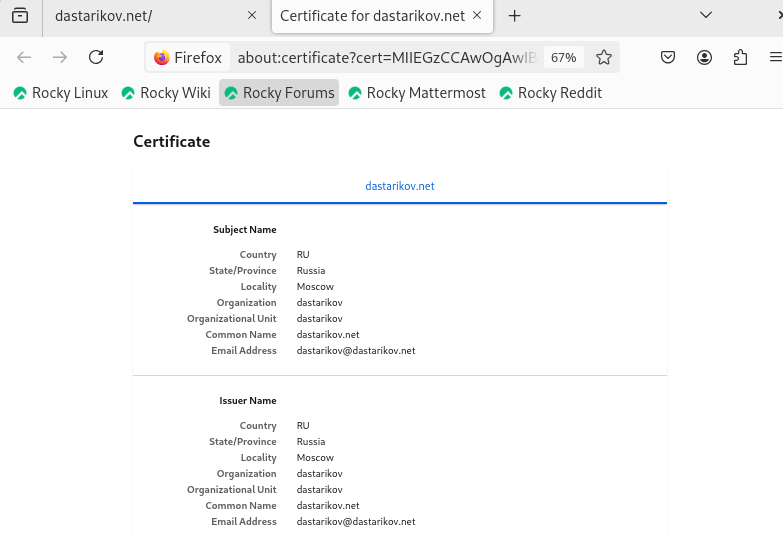
\includegraphics[width=\textwidth]{../images/image06.png}
    \captionof{figure}{Просмотр содержания созданного сертификата.}
    \label{06}
\end{center}

\end{enumerate}
\subsection{Конфигурирование HTTP-сервера для работы с PHP}
\begin{enumerate}
\item Установили пакеты для работы с PHP:
\begin{minted}{bash}
dnf -y install php
\end{minted}
\item В каталоге \texttt{/var/www/html/www.dastarikov.net} заменили файл \texttt{index.html} на \texttt{index.php} следующего содержания:
\begin{minted}{bash}
<?php
phpinfo();
?>
\end{minted}
\item Скорректировали права доступа в каталог с веб-контентом (Рис. \ref{07}):
\begin{minted}{bash}
chown -R apache:apache /var/www
\end{minted}
\item Восстановили контекст безопасности в SELinux (Рис. \ref{07}):
\begin{minted}{bash}
restorecon -vR /etc
restorecon -vR /var/www
\end{minted}

\begin{center}
    \centering
    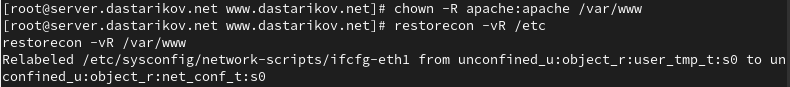
\includegraphics[width=\textwidth]{../images/image07.png}
    \captionof{figure}{Обновление контекста безопасности в SELinux.}
    \label{07}
\end{center}

\item Перезапустили HTTP-сервер:
\begin{minted}{bash}
systemctl restart httpd
\end{minted}
\item На виртуальной машине \texttt{client} в строке браузера ввели название веб-сервера \texttt{www.dastarikov.net} и убедились, что выведена страница с информацией об используемой на веб-сервере версии PHP (Рис. \ref{08}).
  
\begin{center}
    \centering
    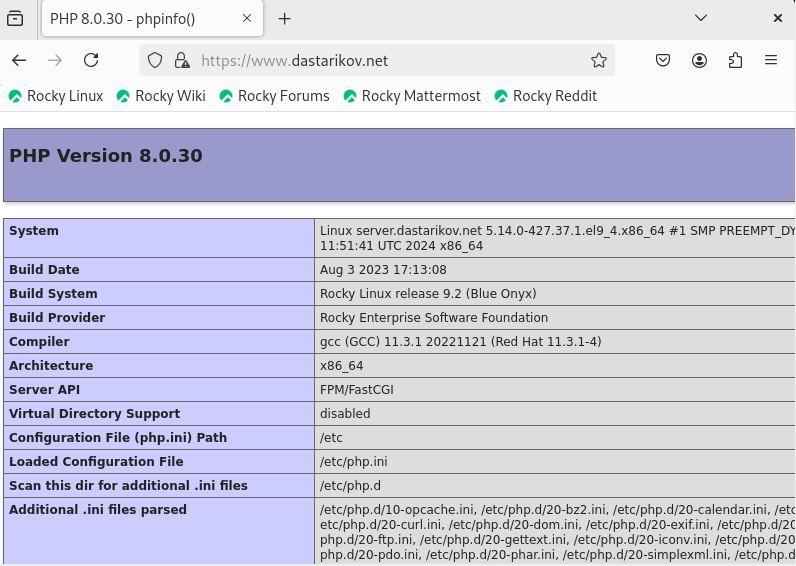
\includegraphics[width=\textwidth]{../images/image08.png}
    \captionof{figure}{Информация об оспользуемой на веб-сервере версии PHP.}
    \label{08}
\end{center}

\end{enumerate}
\subsection{Внесение изменений в настройки внутреннего окружения виртуальной машины}
\begin{enumerate}
\item На виртуальной машине server перешли в каталог для внесения изменений в настройки внутреннего окружения \texttt{/vagrant/provision/server/http} и в соответствующие каталоги скопировали конфигурационные файлы (Рис. \ref{09}):
\begin{minted}{bash}
cp -R /etc/httpd/conf.d/* /vagrant/provision/server/http/etc/httpd/conf.d
cp -R /var/www/html/* /vagrant/provision/server/http/var/www/html
mkdir -p /vagrant/provision/server/http/etc/pki/tls/private
mkdir -p /vagrant/provision/server/http/etc/pki/tls/certs
cp -R /etc/pki/tls/private/www.dastarikov.net.key /vagrant/provision/server/http/etc/pki/tls/private
cp -R /etc/pki/tls/certs/www.dastarikov.net.crt /vagrant/provision/server/http/etc/pki/tls/certs
\end{minted}

\begin{center}
    \centering
    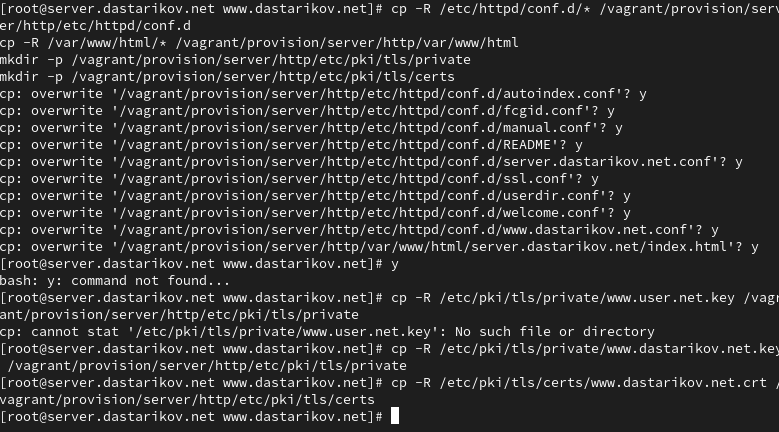
\includegraphics[width=\textwidth]{../images/image09.png}
    \captionof{figure}{Копирование конфигурационных файлов для настройки внутреннего окружения.}
    \label{09}
\end{center}

\item В имеющийся скрипт \texttt{/vagrant/provision/server/http.sh} внесли изменения, добавив установку PHP и настройку межсетевого экрана, разрешающую работать с \texttt{https}.
  \begin{minted}{bash}
#!/bin/bash
echo "Provisioning script $0"
echo "Install needed packages"
dnf -y groupinstall "Basic Web Server"
dnf -y install php
echo "Copy configuration files"
cp -R /vagrant/provision/server/http/etc/httpd/* /etc/httpd
cp -R /vagrant/provision/server/http/var/www/* /var/www
chown -R apache:apache /var/www
restorecon -vR /etc
restorecon -vR /var/www
echo "Configure firewall"
firewall-cmd --add-service=http
firewall-cmd --add-service=http --permanent
firewall-cmd --add-service=https
firewall-cmd --add-service=https --permanent
echo "Start http service"
systemctl enable httpd
systemctl start httpd
  \end{minted}
\end{enumerate}
\section{Выводы}
В результате выполнения лаборатрной работы приобрели практические навыки по расширенному конфигурированию HTTP-сервера Apache в части безопасности и возможности использования PHP.
\end{document}
